\section{Testing Methodology}\label{sec:testing}

This appendix describes the verification and validation framework used to build confidence in each subsystem before advancing to the next integration level, documenting the rationale behind the five-tier progressive approach and the 20 failure scenarios tested before outdoor operations.

The verification and validation strategy draws on V-model principles~\cite{forsberg1991relationship}, where each level of system integration is paired with a corresponding verification activity, and on incremental autonomy practices from safety-critical robotics~\cite{koopman2016challenges}. The resulting five-tier progressive testing framework advances from pure software simulation to full autonomous flight, supported by 74 dedicated test scripts organised across eight categories---including 127 unit tests and 33 automated integration tests---and a stress-testing campaign that exercised 20 failure scenarios before the first outdoor test.

\subsection{V-Model Verification Approach}\label{sec:vmodel}

The classical V-model pairs requirements at each level of decomposition (system, subsystem, component) with a matching verification activity at the same level. In a university project with limited flight days and shared hardware, a strict V-model is impractical; however, its core insight---\emph{verify each integration level before proceeding to the next}---maps directly onto the progressive strategy adopted here.

At the \emph{component} level, individual peripherals (camera, GPS receiver, AI model, MAVLink link) are tested in isolation with dedicated hardware scripts. At the \emph{subsystem} level, bench tests validate the command pipeline (Pi$\to$Cube$\to$actuators) and the sensing chain (camera$\to$inference$\to$coordinate transform) without flight. At the \emph{system} level, passive flight confirms that all subsystems produce coherent results under real outdoor conditions before the software is permitted to issue flight commands. Only after every lower tier passes does the system advance to autonomous operation.

This tiered approach catches integration faults early: a GPS wiring error is discovered at the bench, not at 30\,m altitude; a false-positive rate is quantified during passive flight, not during the first autonomous descent. Each tier constitutes a \emph{gate}---failures must be resolved at the current level before the next is attempted, and the RC kill switch provides an independent hardware-level override at every stage.

\subsection{Five-Tier Progressive Testing}\label{sec:five-tier}

Table~\ref{tab:five-tier} summarises the five tiers and their verification targets.

\begin{table}[H]
\centering
\caption{Five-tier progressive testing framework. Each tier must pass before the next is attempted.}
\label{tab:five-tier}
\small
\begin{tabular}{@{}clp{5.5cm}p{4.0cm}@{}}
\toprule
\textbf{Tier} & \textbf{Environment} & \textbf{What It Verifies} & \textbf{Risk Level} \\
\midrule
1 & SITL simulation (laptop) & State machine logic, path planning, detection pipeline, geofence enforcement & Zero (software only) \\
\addlinespace
2 & Docker Pi test & TFLite model loads on ARM, dependency compatibility, headless operation & Zero (container) \\
\addlinespace
3 & Bench test (Pi + Cube, no props) & MAVLink command ACKs, camera frames, GPS fix, sensing pipeline, servo outputs & Low (grounded) \\
\addlinespace
4 & Passive flight (pilot on RC, Pi logging) & Detection range and rate in real outdoor conditions, FOV and GPS calibration & Medium (no autonomy) \\
\addlinespace
5 & Autonomous flight & End-to-end mission: search, detect, centre, verify, approach, land & High \\
\bottomrule
\end{tabular}
\end{table}

\textbf{Tier~1} uses ArduPilot's Software-in-the-Loop (SITL)~\cite{ardupilot2024} on the development laptop. The same mission orchestrator (\texttt{main.py}), state machine, and detection model execute against a simulated autopilot with GPS noise and vehicle dynamics. A simulated camera extracts FOV-correct sub-images from a georeferenced satellite map, enabling the full detection$\to$estimation$\to$landing pipeline to run without hardware. A 22-test simulation checklist (Section~\ref{sec:stress}) exercises every CLI flag, state transition, and edge case at this tier.

\textbf{Tier~2} uses a Docker container (\texttt{Dockerfile.pi-test}) that replicates the Pi's ARM64 Linux environment with the same lightweight dependency set (\texttt{requirements\_pi.txt}: pymavlink, opencv-headless, numpy, ai-edge-litert). The container loads the TFLite model and confirms that inference produces valid output tensors, catching dependency mismatches before code is deployed to the physical Pi.

\textbf{Tier~3} assembles the Pi, Cube Orange autopilot, and camera on the bench with propellers removed. Three numbered scripts test progressively: \texttt{0a\_cube\_commands} verifies individual MAVLink commands (mode changes, parameter reads, arm pre-checks); \texttt{0b\_bench\_mission} executes the full command sequence (arm, takeoff, waypoint navigation, landing) and confirms every \texttt{COMMAND\_ACK}; \texttt{0c\_feedback\_test} runs the vision-to-GPS pipeline while the operator carries the drone past a dummy, validating the entire sensing chain against hand-measured ground truth.

\textbf{Tier~4} places the assembled drone in the air under full manual RC control. The Pi runs the complete vision pipeline---camera capture, AI inference, coordinate transformation, GPS estimation---but issues \emph{zero flight commands}. All detections are logged with timestamp, pixel coordinates, confidence, altitude, and GPS estimate. Post-flight review of these logs establishes the detection altitude ceiling, false-positive rate, and GPS estimation accuracy under real conditions (wind, lighting, motion blur) before any autonomous behaviour is enabled.

\textbf{Tier~5} enables full autonomy. The drone flies the lawnmower search pattern, detects candidates, centres on them, and presents the live camera feed to the operator for confirmation before initiating the approach sequence. Even at this tier, the operator retains veto authority at the \textsc{Verify} gate and the RC kill switch provides an independent hardware override.

\subsection{Test Script Organisation}\label{sec:test-org}

The test scripts are organised into eight directories, each addressing a distinct verification concern:

\begin{itemize}
    \item \textbf{Hardware} (\texttt{tests/hardware/}, 8 scripts) --- individual component checks: inference benchmarks (standard 50-run and comprehensive multi-model), detection rate under simulated blur, NCNN backend benchmark, GPS satellite tracking, GPS step-by-step health verification, single-frame detection snapshot, and buzzer functionality. These confirm that each peripheral operates correctly before integration.
    \item \textbf{Flight} (\texttt{tests/flight/}, 14 scripts) --- progressive flight tests numbered 0a through 5 by risk level, plus geofence verification scripts (demo, repulsion test), drawing utilities for search area and waypoint definition, and a live map viewer. Lower numbers must pass before higher numbers are attempted; see Section~\ref{sec:five-tier} for the full progression.
    \item \textbf{Diagnostics} (\texttt{tests/diagnostics/}, 5 scripts) --- runtime monitoring tools: a multi-panel connectivity dashboard aggregating all communication links, live Cube telemetry viewer (attitude, GPS, battery), and MJPEG camera streams (standard, threaded, and H.264 variants). The diagnostics dashboard serves as the final go/no-go gate before arming.
    \item \textbf{Calibration} (\texttt{tests/calibration/}, 7 scripts) --- parameter measurement: bench FOV calibration (ruler method), quick single-measurement FOV check, altitude-based FOV at real hover height, lens distortion characterisation (checkerboard $\to$ \texttt{calibration\_data.npz}), GPS ground-truth comparison (CV estimate vs surveyed position), and two focal-length calibration tools (terminal-based and OpenCV GUI).
    \item \textbf{Experiments} (\texttt{tests/day\_1\_experiments/}, 6 scripts) --- structured data collection designed to run passively during Tier~4 manual flights, outputting CSV files for post-flight analysis: altitude sweep, speed sweep, GPS accuracy, GPS drift (CEP50/CEP95), model comparison, and a general detection logger.
    \item \textbf{Laptop} (\texttt{tests/laptop/}, 21 scripts) --- development-only tools: model loading, TFLite and NCNN inspection, synthetic benchmarks, DJI video replay with detection overlay, A/B model comparison, zoom-based detection, path visualisation, NFZ manual testing, and approach/descent simulation. Not used on flight day.
    \item \textbf{Unit} (\texttt{tests/unit/}, 6 files, 127 test functions) --- pytest-based unit tests covering configuration validation, state enum completeness, GPS coordinate transforms, lawnmower pattern generation, vision system initialisation, and GPS utility functions.
    \item \textbf{Automated} (\texttt{tests/automated/}, 7 scripts, 33 test functions) --- extended integration tests: planning edge cases, utility function coverage, vision pipeline tests, geofence optimisation, coverage simulation, and SITL smoke tests.
\end{itemize}

All experiment scripts issue zero flight commands and are safe to run at any time. The CSV output format enables direct import into the analysis presented in Section~\ref{sec:results}.

\begin{figure}[H]
  \centering
  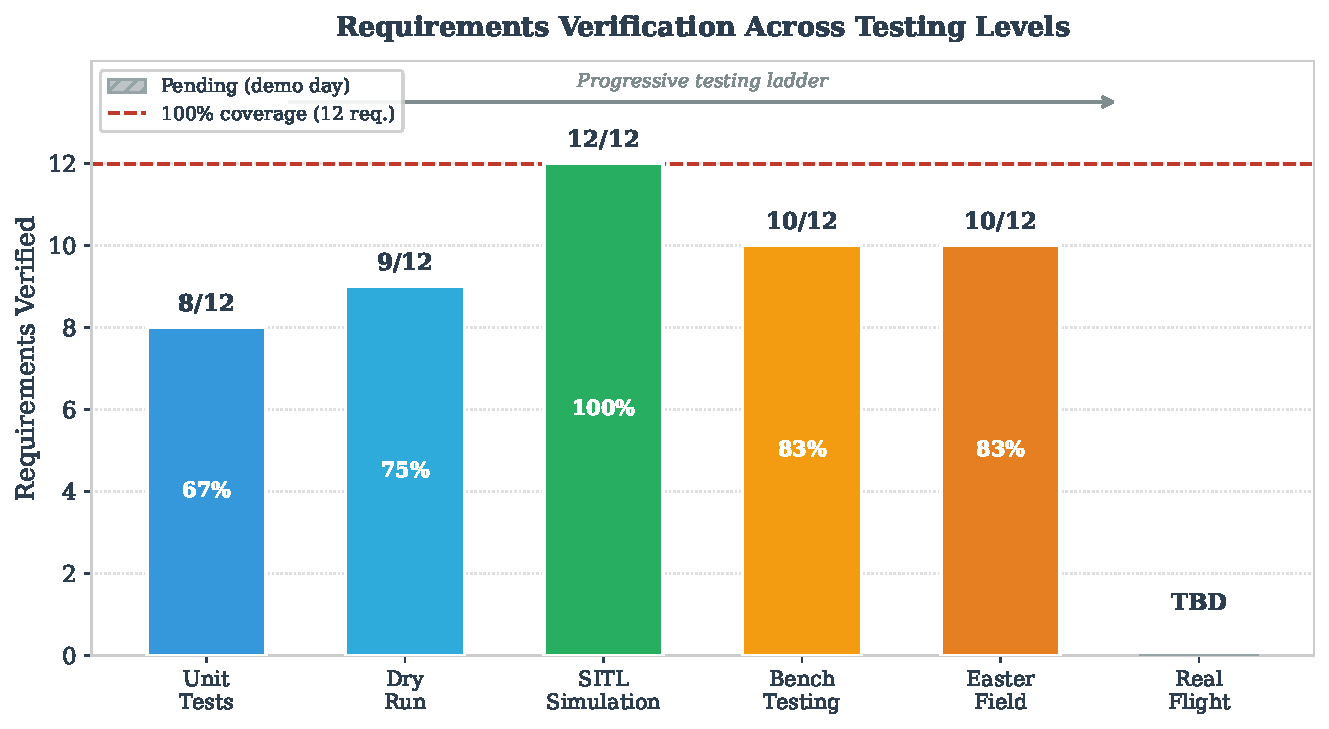
\includegraphics[width=0.85\linewidth]{report/figs/testing_coverage.pdf}
  \caption{Requirements coverage by testing tier.  Each bar shows the number of system requirements (R01--R10) verified at each of the five progressive testing levels (simulation, Docker, bench, passive flight, autonomous flight).  Lower tiers verify a broader set of requirements at lower risk; higher tiers provide operational validation of the most critical flight and mission requirements.  The layered coverage ensures that no requirement depends solely on the highest-risk tier for verification.}
  \label{fig:testing-coverage}
\end{figure}

\subsection{Dry-Run Validation}\label{sec:dry-run}

The \texttt{-{}-dry-run} flag provides an end-to-end state machine walkthrough without requiring hardware, an autopilot connection, or even SITL. When invoked, the system loads the search polygon from the KML file, generates the lawnmower waypoint set, visualises it on a map with geofence boundaries, prints the full mission plan (altitude, speed, waypoint count, estimated time), and walks through the state machine transitions (INIT$\to$SEARCH$\to$VERIFY$\to$LANDING$\to$DONE) to verify that all imports, configuration parameters, and state logic are correct. The output image (\texttt{dry\_run\_pattern.jpg}) provides immediate visual confirmation that the search pattern covers the intended area and respects the SSSI exclusion zone.

Dry-run validation is executed before every flight day as the first item on the preflight checklist and after every code change that modifies state transitions, waypoint generation, or geofence logic. Execution takes under one second and requires only a Python interpreter, making it suitable for rapid iteration during development.

\subsection{DJI Video Analysis}\label{sec:video-analysis}

Real flight footage from a DJI survey drone provided a supplementary validation path between simulation and live flight. The video analysis pipeline replays recorded 4K video at 30\,fps with frame-synchronised SRT telemetry (GPS, altitude, heading) while running the YOLOv8n model on every frame. Each detection is projected from pixel coordinates to GPS coordinates using the calibrated FOV ($\SI{54.4}{\degree}$ HFOV for the cropped $1456 \times 1088$ frame). The pipeline produces scatter plots of estimated target positions, circular error statistics, and a scale bar overlay for visual verification of distance estimates.

An A/B comparison tool switches between model variants during replay, enabling direct evaluation of the baseline and retrained models on identical footage. This analysis informed the decision to retrain on mixed synthetic-plus-real data (Section~\ref{sec:training}) and quantified the GPS estimation accuracy (CEP50 = 2.3\,m, maximum error = 16.5\,m) under real flight dynamics, including the 100--200\,ms GPS timing lag identified during analysis.

\subsection{Stress Testing and Failure Scenarios}\label{sec:stress}

A systematic stress-testing campaign exercised the system's response to 20 failure and edge-case scenarios in SITL simulation prior to outdoor testing. The scenarios were derived from a contingency table---a state-by-failure matrix covering all 15 states against six failure categories (timeout, manual override, GPS loss, camera failure, connection drop, and operator error)---and from the 22-test simulation checklist described below. Table~\ref{tab:stress-results} summarises the results.

\begin{table}[H]
\centering
\caption{Stress test results: 20 failure scenarios tested in SITL.}
\label{tab:stress-results}
\small
\begin{tabular}{@{}p{5.5cm}lp{5.5cm}@{}}
\toprule
\textbf{Scenario} & \textbf{Result} & \textbf{Resolution} \\
\midrule
Camera returns None during search & PASS & Drone completes pattern, returns home \\
Camera fails during verify & FIXED & Added ``CAMERA LOST'' HUD warning \\
GPS fix degrades mid-flight ($<$3D for 5\,s) & PASS & Emergency RTL triggers automatically \\
GPS never acquires fix on ground & PASS & Arm blocked; clear warning printed \\
MAVLink heartbeat lost & PASS & Emergency RTL; GCS failsafe backup \\
Operator timeout at verify (120\,s) & PASS & Auto-reject, search resumes \\
Rapid key presses (M/Y/N/I/X in $<$1\,s) & PASS & Input queue processes FIFO, no crash \\
Detection outside search polygon & PASS & Filtered; not added to queue \\
Duplicate detection of same target & FIXED & Added 5\,m reject radius dedup \\
Queue overflow ($>$50 targets) & FIXED & Hard cap; oldest entries discarded \\
Empty queue after landing & PASS & Resumes search or RTL \\
Geofence breach (drone enters SSSI) & PASS & Immediate MANUAL transition \\
NFZ speed capping at boundary & PASS & Smooth ramp from 3\,m/s to 0.3\,m/s \\
Barometric drift during landing & FIXED & 90\,s absolute timeout + force-disarm \\
Port 8090 in use (stream server) & FIXED & Retry consecutive ports 8091--8099 \\
Servo channel hardcoded (not in config) & FIXED & Moved to config.py parameters \\
Corrupt focus\_area.json & FIXED & Validation + clear error message \\
Transit.json missing & FIXED & Warning + abort with actionable error \\
Home position not set before RTL & FIXED & Guard checks gps\_fix\_ok flag \\
Stale departure point after manual & PASS & Correctly returns to pre-manual position \\
\bottomrule
\end{tabular}
\end{table}

Of the 20 scenarios, 11 passed on the first attempt with the correct automated response already in place. The remaining nine revealed deficiencies---missing timeouts, insufficient input validation, hardcoded parameters, or unclear error messages---that were resolved and re-verified before outdoor testing. No scenario was left unhandled: every failure mode either triggers an automated recovery (RTL, mode change, queue management) or produces an actionable operator warning with a clear next step.

The 22-test simulation checklist provides structured coverage of all operational modes: full autonomous mission (baseline), multi-frame detection confirmation, vision-based centering with GPS averaging, geofence enforcement and disable, manual override workflow, multi-target queue ordering, NFZ speed ramp, out-of-polygon detection filtering, beacon redirect, transit planning, altitude override, dry-run generation, headless mode, code refactoring validation, stream server functionality, confidence threshold tuning, reject radius deduplication, manual-mode queue persistence, rapid input robustness, empty queue handling, and log file integrity.

\subsection{Building Confidence Through Progressive Evidence}\label{sec:confidence-buildup}

The five-tier framework is designed so that each tier produces independently valuable evidence, regardless of whether subsequent tiers are reached.  This property is critical for a university project where flight access is weather-dependent and time-limited: even if autonomous flight is never achieved, the data collected at lower tiers still demonstrates engineering competence and informs the design.

\paragraph{Evidence from Tier~1 (simulation).}
Over 200 simulation runs exercised the state machine, search pattern, and GPS estimation pipeline.  The interactive simulator's configurable noise parameters (GPS drift $\sigma = 0$--5\,m, camera shake 0--15\,px, inference throttle 1--30\,FPS) enabled systematic sensitivity analysis.  The Kalman filter consistently converged within 1\,m of ground truth across all tested noise combinations, outperforming the rolling average estimator under burst-noise conditions.  The 22-test simulation checklist verified every CLI flag, state transition, and edge case, catching nine deficiencies (missing timeouts, hardcoded parameters, unclear error messages) that were resolved before any hardware was involved.

\paragraph{Evidence from Tier~2 (Docker).}
The Docker container test proved that the TFLite model loaded correctly on an ARM64 Linux environment matching the Pi's dependency set, and that the \texttt{ai-edge-litert} package provided a drop-in replacement for the incompatible \texttt{tflite-runtime}.  While this test takes under 30~seconds, it prevented a deployment failure that would have consumed significant debugging time in the field.

\paragraph{Evidence from Tier~3 (bench).}
Bench testing with the assembled hardware produced quantitative calibration data: focal length $f = 5.46$\,mm (correcting a 22\% error from the datasheet default), lens distortion characterisation (RMS = 0.399\,px), and inference benchmarks (206.5\,ms average, 4.8\,FPS, 100\% detection rate at 0.966 confidence).  The three bench scripts exercised the full command pipeline (arm, takeoff, waypoint, land) against the Cube Orange autopilot with propellers removed, confirming that every \texttt{COMMAND\_ACK} was received correctly.  The bench also revealed the IMX296 BGR colour channel issue and the TFLite bounding box coordinate format inconsistency---defects that were invisible to simulation.

\paragraph{Evidence from Tier~4 (passive flight).}
Passive flight with manual RC control and the Pi running the full vision pipeline is designed to produce the most operationally relevant pre-autonomy data: detection rate as a function of altitude, false-positive rate under real outdoor conditions, GPS estimation accuracy against surveyed ground truth, and inference latency under thermal load during sustained operation.  The experiment scripts in \texttt{tests/day\_1\_experiments/} output CSV files structured for direct statistical analysis: \texttt{altitude\_sweep.py} bins detection rate by altitude in 5\,m increments; \texttt{speed\_sweep.py} correlates detection rate with ground speed and blur metrics; \texttt{gps\_accuracy.py} computes CEP statistics against a known dummy position.  This data directly informs the configuration parameters (\texttt{TARGET\_ALT}, \texttt{SEARCH\_SPEED\_MPS}, \texttt{CONFIDENCE\_THRESHOLD}) used in autonomous flight.

\paragraph{Evidence from DJI video replay.}
As a proxy for Tier~4 data obtained before flight access was available, DJI footage from a reconnaissance overflight of the test site was replayed through the identical detection pipeline.  The retrained model achieved 87\% detection rate on frames where the target exceeded $20 \times 20$\,px, with mean confidence 0.82.  GPS estimation produced CEP50 = 2.3\,m.  The video replay also revealed the 100--200\,ms GPS timing lag, which manifested as a systematic along-track bias in position estimates---a phenomenon that would have been difficult to diagnose during a live autonomous flight.

\paragraph{Cumulative confidence.}
The result of this progressive approach is that by the time the system is authorised for autonomous flight, the team holds quantitative evidence for every subsystem's performance envelope.  Failures are discovered at the lowest-risk tier capable of exposing them.  No tier depends on the success of a subsequent tier for its evidence to be valid.  This property---independent value at each level---is the defining characteristic that distinguishes the framework from a simple sequential test plan.

\subsection{Team Roles in the Testing Process}\label{sec:team-testing-roles}

The five-tier testing framework distributed responsibilities across the team to ensure that no single person was a bottleneck for verification progress.

\paragraph{Software development and simulation (Tiers~1--2).}
The software lead was responsible for developing and maintaining the simulation infrastructure, including the interactive simulator, SITL integration, and Docker Pi test.  All simulation test scripts were written, documented, and version-controlled by this team member.  The 22-test simulation checklist and 20-scenario stress test were executed after every significant code change, with results logged in the repository.

\paragraph{Hardware integration and bench testing (Tier~3).}
Hardware assembly, wiring, and bench testing were shared across the team.  The Pi--Cube--camera stack was assembled collaboratively, with each team member responsible for verifying connectivity of specific subsystems (camera, MAVLink link, GPS, servo).  Bench test scripts were designed to be self-contained and executable by any team member without specialised knowledge: each script prints clear pass/fail results and actionable error messages.

\paragraph{Flight operations (Tiers~4--5).}
The qualified pilot retained exclusive authority over RC control and the go/no-go decision.  During passive flight (Tier~4), the pilot flew the drone manually while a second team member monitored the Pi's detection stream on the ground-station laptop and a third recorded observational notes (weather, wind, battery consumption).  During autonomous flight (Tier~5), the pilot's role shifted to safety oversight: monitoring the RC transmitter's kill switch and the Mission Planner telemetry display, ready to intervene if the autonomous system deviated from the expected flight envelope.

\paragraph{Data analysis.}
Post-flight data analysis was conducted by the software lead using the CSV outputs from the experiment scripts.  Detection rate, GPS estimation accuracy, and inference latency statistics were computed and fed back into the configuration file (\texttt{config.py}) for the next flight iteration.  This closed-loop process---fly, measure, tune, repeat---is the mechanism by which the system's operational parameters converge on values validated by real-world evidence rather than simulation assumptions.

\subsection{Comparison with Industry Testing Standards}\label{sec:industry-comparison}

The testing methodology compares favourably with established frameworks for autonomous system verification. NASA's V\&V framework for unmanned aircraft~\cite{nasa2015vv} advocates a progressive increase in operational complexity---simulation, hardware-in-the-loop, limited flight envelope, full mission---which maps directly onto the five tiers described above. The SORA methodology~\cite{jarus2019sora} requires demonstration of failure-mode handling proportionate to the operational risk class; the 20-scenario stress test and contingency table address this requirement by documenting the system's response to every foreseeable failure at every state.

Compared with typical university drone projects, which often proceed directly from simulation to autonomous flight, this project introduces two additional verification tiers---Docker environment testing and passive flight with zero-command CV logging---that substantially reduce the risk of first-flight failures. The passive flight tier is particularly valuable: it generates ground-truth detection data under real outdoor conditions without exposing the system to the risk of autonomous decisions acting on untested detections. The structured experiment scripts produce quantitative metrics (detection rate versus altitude, GPS CEP, model inference latency) that inform configuration tuning before autonomy is enabled, replacing the ad-hoc approach common in time-constrained academic projects.

\subsection{Expected Outcomes from Real Flight Testing}\label{sec:expected-outcomes}

Although full autonomous flight had not been conducted at the time of writing, the simulation and bench-testing data allow quantitative predictions of real-flight performance.  These predictions serve both as design targets and as acceptance criteria: if flight data deviates significantly from these expectations, the deviation identifies a sim-to-real gap that requires investigation.

\paragraph{Detection performance.}
At the nominal search altitude of 35\,m, the camera's ground footprint spans approximately $32 \times 24$\,m.  A standing human (${\sim}1.8$\,m tall) occupies roughly $80 \times 25$\,px in the $1456 \times 1088$ frame---well above the $20 \times 20$\,px threshold at which the retrained model achieved 87\% detection rate on DJI video.  At 4.8\,FPS and 8\,m/s search speed, each ground point appears in approximately 15 consecutive frames, providing multiple detection opportunities per target.  Even if real-flight detection rate drops to 50\% due to motion blur, lighting variation, or thermal effects, each target would still generate 7--8 detections per flyover pass---sufficient to trigger the investigation workflow.  The altitude sweep experiment (\texttt{tests/day\_1\_experiments/altitude\_sweep.py}) is designed to measure the actual detection rate at 5\,m altitude increments, producing the empirical curve needed to set \texttt{TARGET\_ALT} optimally.

\paragraph{GPS estimation accuracy.}
Simulation predicts sub-metre Kalman filter convergence under ideal conditions.  DJI video replay under real conditions yields CEP50 = 2.3\,m.  The operational requirement is to land within 5--10\,m of the target (R07), so the 7.5\,m offset landing provides 5.2\,m of margin against the worst-case CEP50.  The GPS accuracy experiment (\texttt{tests/day\_1\_experiments/gps\_accuracy.py}) would measure the actual estimation error against a surveyed dummy position, closing the loop between predicted and observed accuracy.

\paragraph{Mission duration.}
The lawnmower pattern over the survey polygon at 35\,m altitude with 25\,m strip spacing generates approximately 20 waypoints covering the full area.  At 8\,m/s search speed with B\'{e}zier-smoothed turns, the estimated search time is 8--12~minutes depending on wind.  Adding transit to and from the search area, one investigation cycle (fly to target, hover, verify, return), and the approach/landing sequence, a complete mission is estimated at 15--20~minutes---well within the 25-minute battery endurance of the Hexsoon EDU-450.  The speed sweep experiment (\texttt{tests/day\_1\_experiments/speed\_sweep.py}) would validate the relationship between search speed and detection reliability, confirming whether 8\,m/s is achievable or whether a slower speed is necessary.

\paragraph{Inference under thermal load.}
Bench-measured inference latency (206.5\,ms at room temperature) may increase during sustained outdoor operation as the Pi~5's SoC reaches thermal throttling temperature (${\sim}85^{\circ}$C).  The benchmark script (\texttt{tests/hardware/benchmark.py}) runs 50 consecutive inference passes and reports the latency trend across the run.  During a 15-minute mission, the Pi processes approximately 4\,300 frames; if thermal throttling increases latency by 50\% (to ${\sim}310$\,ms, or 3.2\,FPS), the effective detection window per target drops from 15 to 10 frames---still sufficient for reliable triggering.  A passive heatsink or brief inference pauses between waypoints are available mitigations if thermal degradation is observed.

\subsection{Preflight Checklist}\label{sec:test-preflight}

A structured preflight checklist is executed before every flight session, covering four domains:

\begin{enumerate}
    \item \textbf{Hardware inspection} --- battery voltage and capacity, propeller security, camera lens cleanliness, antenna connections, wiring integrity.
    \item \textbf{Software verification} --- correct code version pulled from the repository, AI model file verified (\texttt{best.tflite} checksum), configuration parameters reviewed (altitudes, speeds, geofence coordinates, search polygon). A dry-run is executed to confirm the search pattern and geofence visualisation.
    \item \textbf{Communication links} --- mavproxy bridge running with dual UDP outputs, Mission Planner connected via TCP, MJPEG video stream accessible in the ground station browser, RC transmitter bound and responsive.
    \item \textbf{Safety systems} --- RC kill switch tested (mode switch to STABILIZE), geofence boundaries loaded and visualised, link-loss timeout configured, return-to-home altitude set.
\end{enumerate}

The diagnostics dashboard (\texttt{diagnostics.py}) provides a single-screen summary of all communication links, camera status, GPS fix quality, and battery level, serving as the final go/no-go gate before arming. The complete checklist, including per-state contingency actions, is maintained as a printable document (\texttt{docs/FLIGHT\_DAY\_CHECKLIST.md}) designed to be followed top-to-bottom without requiring prior system knowledge.
